\documentclass[letterpaper]{article}


\usepackage{aaai}
\usepackage{times}
\usepackage{helvet}
\usepackage{courier}
\usepackage{amsmath}
\usepackage[linesnumbered,ruled,vlined]{algorithm2e}
\usepackage{graphicx}

\def\und#1{\noindent{\bf #1}:}
\def\citep#1{\cite{#1}}
\def\citet#1{\citeauthor{#1} (\citeyear{#1})}
\def\FFRISKY{{\tt DeFAULT}}
\def\default{{\tt DeFAULT}}
\def\goalie{{\tt Goalie}}
\renewcommand{\baselinestretch}{0.99}

\renewcommand\floatpagefraction{1} \renewcommand\topfraction{1}
\renewcommand\bottomfraction{1} \renewcommand\textfraction{0}
\renewcommand{\dbltopfraction}{1}
\renewcommand{\dblfloatpagefraction}{1}
\setcounter{totalnumber}{50} \setcounter{topnumber}{50}
\setcounter{bottomnumber}{50} \setcounter{dbltopnumber}{50}

  
\newenvironment{packed_enum}{
\begin{enumerate}
  \setlength{\itemsep}{1pt}
  \setlength{\parskip}{0pt}
  \setlength{\parsep}{0pt}
}{\end{enumerate}}

\newenvironment{packed_itemize}{
\begin{itemize}
  \setlength{\itemsep}{1pt}
  \setlength{\parskip}{0pt}
  \setlength{\parsep}{0pt}
}{\end{itemize}}
\nocopyright



\title{Reactive, Proactive, and Passive Learning about Incomplete Actions}
\author{Christopher Weber \and Daniel Bryce\\
christopherweber@hotmail.com, daniel.bryce@usu.edu\\
Department of Computer Science\\
Utah State University}

\begin{document}
%\nocopyright
\maketitle

\begin{abstract}
Agents with incomplete knowledge of their actions can either plan around the
incompleteness, learn by querying a domain expert, or learn through
trial and error.  In deciding what to learn, an agent must consider whether an
incomplete action feature is relevant to achieving its goals.  In deciding how
to learn an action feature, the agent can i) try to execute the action and
{\em passively} observe the outcome, ii) {\em react} by querying a domain expert
when it fails to learn by passive observation, or iii) {\em proactively} query a
domain expert prior to executing the action.  The challenge is that by learning about
incomplete action features an agent may determine its plan will fail and
re-plan, and thus change which action features are relevant to achieving it
goals.  We desire agents that can ask as few questions as
possible in achieving their goals.

We present a number of strategies for i) planning with incomplete knowledge of
actions to identify relevant incomplete action features (preconditions and
effects), ii) reasoning about plan failure explanations to identify which
features will be learned passively or proactively, and iii) techniques for
diagnosing action failures to reactively learn about actions when passive
learning fails.  We test the following configurations of our agent: i) learning
only passively and asking no questions; ii) asking questions and re-planning
until the plan is guaranteed to succeed; iii) planning, acting until the plan
fails, diagnosing the failure, and re-planning; and iv) while diagnosing
failures, proactively querying about a subset of the future action features that are likely to cause failures. 
We find that passive learning alone can lead to dead-ends, perfecting a plan
prior to execution requires many questions, and balancing passive learning with
reactive learning strikes a good balance between avoiding dead-ends and
minimizing the number of questions.


% consider what
% information is relevant to achieving its goals (goal-directedness) and what
% information can be gleaned from prior plan failures to avoid future failures
% (failure-directedness).  Upon determining which information is relevant, the
% agent can either choose to ignore it (hoping that it will not cause its plans
% to fail), choose to passively learn it by applying the action, reactively learn
% about (diagnose) it when it may have caused plan failure, or actively query the
% domain expert before it causes failure.  
% We present and evaluate several approaches to learning about incomplete actions
% in model-lite planning scenarios that seek to reduce the number of actions
% executed by agents to achieve their goals, the number of failure
% driven re-planning episodes required, and the number of questions posed to a
% domain expert.  Our work addresses the familiar reinforcement learning issue of
% exploitation and exploration by using plans and a domain expert to simplify and
% focus exploration.  We show that asking plan and failure relevant questions of a
% domain expert in the event of plan failure and otherwise learning passively outperforms i) purely
% passive learning (by re-planning less) and ii) purely goal-directed learning (by
% asking fewer questions). 

\end{abstract}

\section{Introduction}

% Average employees should be able to perform their assigned duties with minimal
% guidance from their superiors.  Excellent employees can perform new duties
% involving potentially unfamiliar actions. While it is expected that questions
% may arise during the new task, a deluge of questions will be met with
% animosity.  Thus, an employee should learn about the task as they proceed, but
% only ask the questions necessary to avoid catastrophic failure or unreasonable
% delay in completing the task.  Building autonomous agents that behave like an
% excellent employee requires the ability to plan with incomplete knowledge of
% actions, learn about the actions whenever possible, and identify relevant
% questions that can be asked of domain experts.  

Knowledge engineering \citep{ickeps09} and machine learning
\citep{arms,DBLP:conf/aaai/OatesC96} have been applied to constructing
representations for planning, but pose intensive human and/or data requirements,
only to leave a potential mismatch between the environment and model
\citep{modellite}.  Recently, we \cite{bryce-icaps11} showed that instead of
placing effort upon making domains complete it is possible for our planner
\default{} to plan with incomplete knowledge of an agent's action descriptions
(i.e., plan around the incompleteness).  Agents executing such robust plans fail and re-plan less often
 than agents that ignore
incompleteness when planning \citep{DBLP:conf/aips/ChangA06}.  While
we demonstrated that planning in incomplete domains can
help agents passively learn about domains, we ignore cases where domain
experts are available to help engineer the agent's knowledge.  We extend our
prior work \citep{bryce-icaps11} to
consider agents that can query a domain expert, as in instructable computing
\citep{mable}, but must carefully select their questions.

Selecting questions is a problem that has been studied in problems such as
preference elicitation \citep{DBLP:conf/aaai/Boutilier02}, machine learning
\citep{AICPub1812:2011}, and model-based diagnosis
\citep{deKleer:1992:CDS:140524.140531}.  
Incomplete action knowledge is unique in that plans have rich causal structure
that makes questions highly coupled, and frequent re-planning can change which
questions are relevant.  


We seek to understand whether asking questions is at all necessary, and if so,
how to select the fewest questions.  Agents that passively learn by trial and
error can reach scenarios where it is impossible to learn about actions that impact goal
achievement without asking questions. For example, an agent might apply an
action with $n$ possible preconditions that are unsatisfied in the current
state, and to know why the action failed (i.e., which of the possible
preconditions are actual preconditions), it would need to apply the action again in 
several different states (some of which may be unreachable) to isolate the
problem. Instead, the agent could reactively query the domain expert to determine the problem, or prior to
executing the action proactively query the domain expert.  Reactive agents take
a risk that  the action will not fail (i.e., the possible preconditions
are not required), and proactive agents will not risk failure.  


We systematically test different approaches to planning, acting, and learning
with incomplete actions that:
\begin{enumerate}
\item Ask no questions, but learn passively. 
\item Proactively ask questions and re-plan until a plan is guaranteed to
succeed.
\item Reactively ask questions only when learning passively insufficiently
learns about an action.
\item  Proactively ask about
highly impactful future failures and 3.
\end{enumerate}
We find that the first approach can lead to dead-ends where the agent fails or
because of its passive learning it is incapable of formulating an effective
plan.  The second technique is highly successful, but asks many questions.  The
third, asks fewer questions and overcomes the problems of passive learning.  The
fourth asks more questions but reaches
dead-ends less often.

Our presentation includes a discussion of incomplete STRIPS, belief maintenance
and planning in incomplete domains, strategies for selecting questions, an empirical evaluation in several domains,
related work, and a conclusion.

\section{Background \& Representation}\label{sec:background}

Incomplete STRIPS relaxes the classical STRIPS model to allow for
possible preconditions and effects \citep{Garland02}.  
Incomplete STRIPS domains are identical to STRIPS domains, with the exception
that the actions are incompletely specified.  Much like planning with incomplete
state information \citep{bonet00planning}, the action incompleteness is not
completely unbounded.  The preconditions and effects of each action can be any
subset of the propositions $P$; the incompleteness is with regard to a lack of
knowledge about which of the subsets correspond to each precondition and effect.        

\und{Incomplete STRIPS Domains} An incomplete STRIPS domain ${D}$  defines the
tuple ($P$, ${A}$, $I$, $G$, $F$), where: $P$ is a  set of propositions, ${A}$
is a set of incomplete  action descriptions, $I \subseteq P$ defines a set of
initially true  propositions, $G \subseteq P$ defines the goal propositions, and
$F$ is a set of propositions describing incomplete domain features. Each action
${a} \in {A}$ defines $pre({a}) \subseteq P$, a set of known preconditions,
$add({a}) \subseteq P$, a set of known add  effects, and $del({a}) \subseteq P$,
a set of known delete effects.   The set of incomplete domain features $F$ is
comprised of propositions of the form $pre({a}, p)$, $add({a}, p)$, and
$del({a}, p)$, each indicating that $p$ is a respective possible precondition, add effect, or
delete effect of $a$.

Consider the following incomplete domain: 

$P = \{p, q, r, g\}$, 

${A} =
\{{a}, {b}, {c}\}$, 

$I = \{p, q\}$, 

 $G= \{g\}$, and 
 
 $F = \{pre(a, r), add(a, r),
del(a, p),del(b, q), pre(c, q) \}$.  

The
known features of the actions are defined: 

 $pre({a}) = \{p, q\}$, 
 
 $  pre({b}) =
\{p\},  del(b) = \{p\}, add({b}) = \{r\}$, and

  $ pre({c}) =
\{r\},  add({c}) = \{g\}$. 

An interpretation $F^i \subseteq F$ of the incomplete STRIPS domain
defines a STRIPS domain, in that every feature $f \in F^i$
indicates that a possible precondition or effect is a respective known
precondition or known effect; those features not in $F^i$ are
not preconditions or effects.   



\und{Incomplete STRIPS Plans} A plan $\pi$ for ${D}$ is a sequence of
actions, that when applied, {\em can lead} to a state where the goal is
satisfied.  A plan $\pi = ({a}_0,  ..., {a}_{n-1})$ in an incomplete
domain ${D}$ is a sequence of  actions, that corresponds to the {\em
optimistic} sequence of states $(s_0, ...,  s_n)$, where $s_0 = I$,
$pre({a}_t) \subseteq s_t$ for $t = 0,...,  n$, $G \subseteq s_n$,
and $s_{t+1} = s_t \backslash del({a}_t)  \cup
add({a}_t) \cup \{p | add(a, p) \in
F\}$ for $t = 0,...,
n-1$.

For example, the plan $({a}, {b}, {c})$ corresponds to the
state sequence $(s_0 = \{p, q\}, s_1 = \{p, q, r\}, s_2 = \{q, r\}, s_3 = \{q,
r, g\})$, where the goal is satisfied in $s_3$.  We note that $r \in s_1$ even
though $r$ is only a possible add effect of $a$; without listing $r$ in $s_1$,
the known precondition of $b$ would not be satisfied.  While it is possible that
in the true domain $r$ is not an add effect of $a$, in the absence of contrary
information we optimistically assume $r$ is an add effect so that we can
synthesize a plan.   Pessimistically disallowing such plans is admissible, but
constraining, and we prefer to find a plan that may work to finding no plan at
all.  Naturally, we prefer plans that succeed under more interpretations.

\section{Belief Maintenance \& Planning}

An agent can act, ask questions, and plan.  Acting and asking a question provide
observations of the incomplete domain that can be learned from, and planning
involves predicting future states (in the absence of observations).  In the following, we discuss how
observations can be filtered to update an agent's knowledge $\phi$ (defined over
the literals of $F$), and what can be assumed about predicted states
(when taking knowledge into account).  We denote by $d(\pi)$ a plan's failure
explanations/diagnoses, which is represented by a propositional sentence over
$F$.

We use $\phi$ to reason about actions and
plans by making queries of the form $\phi \models
add({a}, p)$ (``Is $p$ a known add effect of
${a}$?''), $\phi \not\models add({a}, p)$ and $\phi
\not \models \neg add({a}, p)$  (``Is $p$ a
possible/unknown add effect of ${a}$?''),  or $\phi \models d(\pi)$ (``Is the
current knowledge consistent with every interpretation where $\pi$ is guaranteed
to fail?'').  It is often the case that it is unknown if an incomplete feature
$f \in F$ exists in the true domain that is consistent with $\phi$ (i.e., $\phi \not\models f$ and $\phi \not\models
\neg f$), and we denote this by ``$\phi?f$''.


\begin{figure*}[t]\centering
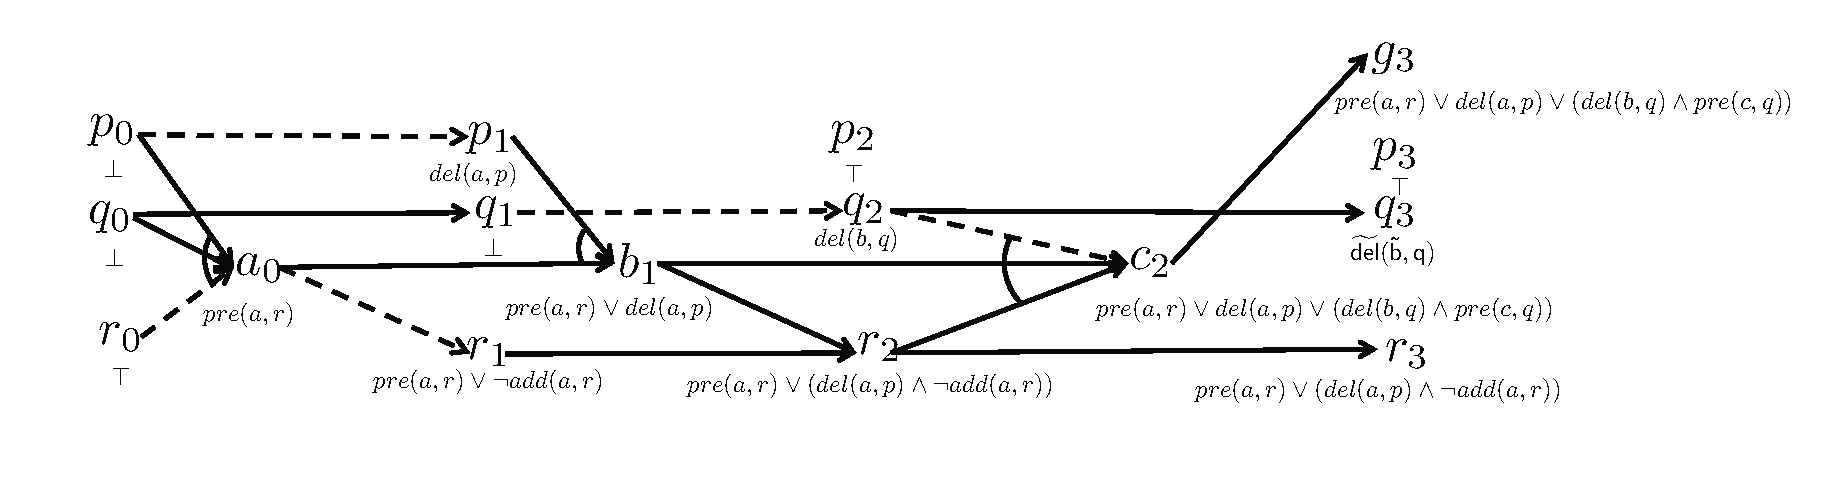
\includegraphics[width=1\linewidth]{WeberBryceICAPS11Fig1.eps}\caption{\label{fig:example}
Labeled Plan}
\end{figure*}


\und{Filtering Observations} An agent that acts in incomplete STRIPS domains
will start with no knowledge of the incomplete features (i.e., $\phi = \top$),
however, taking actions provides state transition observations of the form $o(s,
a, s')$, and asking questions (i.e., ``Is $f$ true or false?'') provides
observations of the form $f$ or $\neg f$.  Thus the function ${\tt filter}$
returns the updated knowledge $\phi'$ after an observation, and is
defined:

\begin{align*}
{\tt filter}(\phi, f) & = \phi \wedge f \\
{\tt filter}(\phi, \neg f) & = \phi \wedge \neg f \\
{\tt filter}(\phi, o(s, a, s)) & = \phi \wedge ((fail \wedge o^-) \vee  o^+)\\
{\tt filter}(\phi, o(s, a, s')) & = \phi \wedge  o^+, s \not= s'
\end{align*}
 where 
\begin{eqnarray*}
o^- &=& \bigvee\limits_{\substack{pre({a},p) \in 
F:\\ p \not\in s} } pre({a},p) 
\label{eqn:update1} \\
o^+ &=& o^{pre} \wedge o^{add} \wedge o^{del}\label{eqn:update2}\\
o^{pre} &=& \bigwedge\limits_{\substack{pre({a},p)
 \in F:\\ p \not\in s} }\neg pre({a},p)
 \label{eqn:update3}  \\
\end{eqnarray*}

\begin{eqnarray*}
o^{add} &=& \bigwedge\limits_{\substack{add({a},p) \in 
F:\\ p\in s'\backslash s} }add({a},p) 
  \wedge \bigwedge\limits_{\substack{add({a},p) \in 
  F: \\ p \not\in  s\cup s'}} \neg 
  add({a},p)   \label{eqn:update4}\\
o^{del} &=& 
\bigwedge\limits_{\substack{del({a},p) \in {\sf
F}: \\p \in s \backslash s'}}
del({a},p)  \wedge
\bigwedge\limits_{\substack{del({a},p)
\in F:\\ p \in s\cap s'}}\neg
del({a},p)  \label{eqn:update5}
\end{eqnarray*}
\noindent We assume that the state will remain unchanged upon executing
an action whose precondition is not satisfied, and because the
state is observable, ${\tt filter}(\phi, o(s, a, s))$ references the case where
the state does not change and ${\tt filter}(\phi, o(s, a, s'))$, the case where
it changes.  If the state does not change, then either the action failed
($o^-$) and one of its unsatisfied possible preconditions is a precondition  or
the action succeeded ($o^+$).  We use the $fail$ literal to denote
interpretations under which a plan failed because it is not always observable
that the plan has failed. If the state changes, then the agent knows that the
action succeeded. If an action  succeeds, the agent learns that i) each possible
precondition that was not satisfied is not a precondition ($o^{pre}$), ii) each possible add effect that appears in the successor but not the predecessor state is an add effect and each that does not appear in either state is not an add 
effect ($o^{add}$), iii) each possible delete effect that appears in the
predecessor but not the successor is a delete effect and each that  appears in both states is
not ($o^{del}$).




\und{Planning} We label predicted state propositions and actions with domain
interpretations that will respectively fail to achieve the proposition or fail
to achieve the preconditions of an action.  That is, labels indicate the cases
where a proposition will be false (i.e., the plan fails to establish the
proposition). Labels $d(\cdot)$ are represented as  propositional sentences over
$F$ whose models correspond to failed domain interpretations.


Initially, each proposition $p_0 \in s_0$, in the state from which a plan is
generated, is labeled $d(p_0) = \perp$ to denote that there are no
interpretations in the current state where a proposition may be false (the state is fully-observable), and each $p_0 \not\in
s_0$ is labeled $d(p_0)=\top$ to denote they are known false.
For all $t \geq 0$, we define:

 \begin{align}
%\label{eqn:actlabel}
\notag d({a}_t) =&  
d(a_{t-1}) \vee\hspace*{-.5cm} \bigvee\limits_{\substack{p \in pre(a)
\;\text{or}\;\\\phi \models pre(a, p)}}\hspace*{-.5cm} d(p_t) \vee
\hspace*{-.5cm}\bigvee\limits_{\substack{p : \phi?pre(a, p)}}
\hspace*{-.5cm}(d(p_t)\wedge pre({a}_t, p)  ) \notag %& : { t $\geq$ 1 }
%\end{array}\right.
\\
\notag\hspace*{-.1cm}d(p_{t+1}) &= \left\{
\begin{array}{l@{\;}l@{\;}r}
d(p_t) \wedge d({a}_t) & : p \in add({a}_t) \\ 
 & \;\text{or}\; \phi \models add({a}_t, p)\\
d(p_t) \wedge (d({a}_t) \vee & : \phi?add({a}_t,p)\\
 \hspace*{1.25cm} \neg add({a}_t, p)) \\  
\top & : p \in del({a}_t)\\
 & \;\text{or}\; \phi \models del({a}_t,p)\\
d(p_t) \vee  del({a}_t, p)  &: \phi?del({a}_t, p)\\
d(p_t) & : {otherwise} 
\end{array}
\right. 
\end{align}

\noindent where $d({a}_{-1}) = \perp$. The intuition behind the label
propagation is that an action will fail  in the
domain interpretations $d({a}_t)$ where a prior action failed, a known
precondition is not satisfied, or a possible precondition is not satisfied. As defined for
$d(p_{t+1})$, the plan will fail to achieve a proposition at time $t+1$ in all
interpretations where i) the plan fails to achieve the proposition at time $t$ and the action fails, ii) the plan fails to achieve the proposition at
time $t$ and the action fails or it does not add the proposition in the
interpretation, iii) the action deletes the proposition, iv) the plan fails to
achieve the proposition at time $t$ or in the interpretation the action deletes
the proposition, or v) the action does not affect the proposition and  prior
failures  apply.             

A consequence of our definition of action failure is that each action fails if
any prior action fails.  This definition follows from the semantics that the
state becomes undefined if we apply an action whose preconditions are not
satisfied.  While we use this notion in plan synthesis, we explore the semantics
that the state does not change (i.e., it is defined) upon failure when acting in
incomplete domains.  The pragmatic reason that we define action failures in this
manner is that we can determine all failed interpretations affecting a plan $d(\pi)$,
by defining $d(\pi) = d({a}_{n-1}) \vee \bigvee_{p \in G} d(p_n)$ (i.e.,
failure to execute an action is propagated to a
failure to achieve the goal). 


For example, consider the plan depicted in Figure \ref{fig:example}.  The
propositions in each state and each action at each time are labeled by the
propositional sentence below it. The edges in the figure connecting the
propositions and actions denote what must be true to successfully execute an
action or achieve a proposition.  The dashed edges indicate that action
incompleteness affects the ability of an action or proposition to support a
proposition.  For example, $a$ possibly deletes $p$, so the edge
denoting its persistence is dashed.  The propositional sentences  $d(\cdot)$
below each proposition and action denote the domain interpretations where a
action will fail or a proposition will not be achieved.  For example,
$b$ at time one, $b_1$, will fail if either
$pre(a, r)$ or $del(a,
p)$ is true in the interpretation.  Thus, $d(\pi) = 
pre(a, r) \vee  del(a, p) \vee (del(b, q) \wedge pre(c, q))$ and any domain interpretation satisfying
$d(\pi)$ will fail to execute the plan and achieve the goal.


% For example, our plan example from the previous
% section has the failure explanation label $d(\pi) = 
% pre(a, r) \vee  del(a, p) \vee (del(b, q) \wedge pre(c, q))$.

\und{Incomplete Domain Relaxed Plans} The \default{} planner
\citep{bryce-icaps11} guides its expansion of plans that are labeled with
failure explanations by computing relaxed plans with failure explanations.   Finding a
relaxed plan that attempts to minimize failure explanations involves propagating
failed interpretation labels in a planning graph.  Propagating labels relies on
selecting an action to support each proposition, and we select the supporter
$a_{t+k}(p)$ at step $k$ of the planning graph for state $s_t$ with the
fewest failed interpretations, denoted by its label $\hat{d}(a_{t+k}(p))$.

A relaxed planning graph with propagated labels is a layered graph of sets of
vertices of the form $({\cal P}_t, {\cal A}_t, ..., {\cal A}_{t+m},
{\cal P}_{t+m+1})$. The relaxed planning graph built for a state
${s}_t$ defines ${\cal P}_t = \{{p}_t | p \in {s}_t\}$,
${\cal A}_{t+k} = \{ {a}_{t+k} | \forall_{p \in {pre}({a})}
{p}_{t+k} \in {\cal P}_{t+k}, {a} \in {A} \cup A(P)\}$, and
${\cal P}_{t+k+1} = \{p_{t+k+1} | {a}_{t+k} \in {\cal A}_{t+k}, p
\in {add}({a}) \cup \{p | \phi\not\models\neg add({a}, p)\}$, for $k
= 0, ..., m$.  Much like the successor function used to compute next states, the
relaxed planning graph assumes an optimistic semantics for action effects by
adding possible add effects to proposition layers, but, as we will explain
below, it associates failed interpretations with the possible adds.

 Each planning graph vertex has a label, denoted $\hat{d}(\cdot)$.  The failed
 interpretations $\hat{d}(p_t) $ affecting a proposition are defined such that
 $\hat{d}(p_t) = d(p_t)$, and for $k \geq 0$,
\begin{align}
\hat{d}({a}_{t+k}) &= \hspace*{-.2cm}
\bigvee\limits_{\substack{p \in pre({a}) \;\text{or}\;\\ \phi\models
pre(a, p) }} \hspace*{-.2cm}
\hat{d}(p_{t+k}) \vee \hspace*{-.25cm} \bigvee\limits_{\phi?pre(a, p)}
\hspace*{-.25cm} (\hat{d}(p_{t+k})  \wedge pre({a}, p) )\notag\\ \notag
\hspace*{-.6cm} \hat{d}(p_{t+k+1}) &= \left\{\begin{array}{l@{\;}l@{\;}r}
\hat{d}({a}_{t+k}(p)) & : p \in add(a_{t+k}(p))\\ & \;\text{or}\; \phi\models
add(a_{t+k}(p), p)\\
\hat{d}(a_{t+k}(p)) \vee& : \phi?add(a_{t+k}(p), p)\\
\neg add(a_{t+k}(p), p)
\end{array}\right. \hspace*{-.1cm}\label{eqn:hprop}
\end{align}
% Propositions in the planning graph initially have the same faults associated
% with them as in state $\tilde{s}_t$ and are defined by $d(\cdot)$.
Every action in every level $k$ of the planning graph will fail in any
interpretation where their preconditions are not supported.  A proposition will
fail  to be achieved in any interpretation where the chosen supporting action
fails to add the proposition.

% We note that the rules for propagating labels in the planning graph differ from
% the rules for propagating labels in the state space.  In the state space, the
% action failure labels include interpretations where any prior action fails.  In
% the relaxed planning problem, the action failure labels include only
% interpretations affecting the action's preconditions, and not prior actions; it
% is not clear which actions will be executed prior to achieving a proposition
% because many actions may be used to achieve other propositions at the same time
% step.

%\und{Choosing Supporters} While only a single action or noop may be required to support a proposition, using multiple supporters can increase the number of incomplete domain interpretations that support it (by ensuring that not all sources of support are subject to the same faults).  We wish to select a set $\hat{\cal S}_{t+k}(p) \subseteq \{\tilde{a} \in \hat{\cal A}_{t+k} | p \in \text{add}(\tilde{a}) \cup \widetilde{\text{add}}(\tilde{a})\}$ to define a most preferred $\hat{d}_{t+k+1}(p)$ (i.e., have fewer explanations of failure).  We use a greedy algorithm to incrementally add actions to $\hat{\cal S}_{t+k}(p)$, and check if $\hat{d}_{t+k+1}(p)$ is improved.
%
%The greedy algorithm proceeds as follows.  We consider all singleton sets of actions, and select the most preferred (having the fewest failure explanation models or prime implicants, and breaking ties by selecting noop actions).  To the most preferred action set, we add each action and determine the most preferred, two element action set.  If none of the two element action sets are more preferred than the best single action set, we define $\hat{\cal S}_{t+k}(p)$ as the best single action set.  Otherwise, the algorithm continues to extend the best action set with one action at a time until it cannot find a more preferred action set (by counting models or prime implicants).
%
% alternative definitions (one for each possible supporter) of the set $\hat{\cal S}_{t+k}(p)$, and select the supporter that has the most preferred definition of  $\hat{d}_{t+k+1}(p)$ (breaking ties by first preferring noop actions and second preferring actions whose first appearance in the planning graph is earliest).  With a single element in $\hat{\cal S}_{t+k}(p)$, we evaluate all single element extensions of the set (making it a two element set), choosing the extension that most improves the measure of $\hat{d}_{t+k+1}(p)$ (depending on the chosen measure, either reducing the number of models, or prime implicants); if no extension improves the measure, then the algorithm terminates and returns $\hat{\cal S}_{t+k}(p)$ with a single element.  In our implementation, we allow at most two supporters per proposition, but it is possible to allow an arbitrary number of supporters in this fashion by extending the set of supporters greedily until no new extension improves its measure.
%



%\und{Heuristic Computation}
 The relaxed planning graph expansion terminates
at the level $t+k+1$ where the goals have
been reached at $t+k+1$. The $h^{\sim FF}$ heuristic makes use of the chosen
supporting action $a_{t+k}(p)$ for each proposition that requires support in the relaxed
plan, and, hence, measures the number of actions used while attempting to
minimize failed interpretations.  The failure explanation of the relaxed plan is
defined by $d(\hat{\pi}) = \bigvee\limits_{p \in G} \hat{d}(p_{t+m+1})$.  We
also use the $h^{FF}$ heuristic \citep{hoffmann:nebel:jair-01} for comparison,
which does not select supporting actions based on failure explanations.


\section{Passive Learning}

% We describe several approaches to formulating questions for a domain expert in
% incomplete domains, which include asking all possible questions in an uninformed
% manner, asking no questions but learning by trial and error, and using plans to
% select goal directed questions. We discuss the approaches by increasing
% sophistication and follow with an empirical evaluation.
% 
% \und{Uninformed QA} Uninformed QA (UQA) is the strategy taken by an agent that
% cannot or will not plan or act under uncertainty and thus must ask the domain expert about each incomplete
% feature of the domain without regard to its relevance to goal achievement.  As
% such, uninformed QA based agents will ask a set of questions $Q_{F} = F$ about
% every feature in $F$, formulate a classical plan, and execute the plan.

A passive learner would rather act
under uncertainty and ask no questions of the domain expert.  Passive learning
agents are potentially reckless because 
they apply actions whose preconditions may be unsatisfied.  

Using their knowledge $\phi$, it is possible to determine if the next action in
a plan, or any subsequent action, can or will fail.  If  $\phi \wedge d(\pi)$ is
satisfiable, then $\pi$ {\em can} fail, and if $\phi \models d(\pi)$,
then $\pi$ {\em will}  fail.  
% The agent will execute an action if it may not
% fail, but will re-plan if any action is guaranteed to fail.  If
% \goalie{} determines that its next action will fail, or a prior action failed ($\phi \models fail$), then
% it will re-plan.  \goalie{}  uses $\phi$ to modify the actions during
% re-planning by checking for each incomplete domain feature $f \in {\sf
% F}({D})$ if $\phi \models f$ or if $\phi \models \neg f$.  Each such
% literal entailed by $\phi$ indicates if the respective action has the possible
% feature as a known or impossible feature; all other features remain as possible
% features.
Algorithm \ref{alg:replan} is the strategy used by the passive learning agent. 
The algorithm involves initializing the agent's knowledge and plan (line 1), and then while
the plan is non-empty and the goal is not achieved (line 2) the agent proceeds
as follows.  The agent selects the next action in the plan (line 3) and
determines if it can apply the action (line 4).  If it applies the action, then
the next state is returned by the environment/simulator (line 5) and the agent
updates its knowledge (line 6) and state (line 7),
otherwise the agent determines that the plan will fail (line 9).  If the plan
has failed (line 11), then the agent forgets its knowledge of the plan failure
by projecting over $fail$ (line 12) and finds a new plan using its new knowledge
(line 13).

For example, the passive agent might observe the state transition $o_1
= o(\{p,q\}, a, \{p,q\})$ upon executing $a$, and $\phi' = {\tt filter}(\phi,
o_1) = \neg del(a, r)$.  The agent must re-plan because $\phi' \models d(\pi)$.

% \goalie{} is not hesitant to apply actions that may fail because trying actions
% is its only way to learn about them.  However, \goalie{} is able to determine
% when actions will fail and re-plans.  More conservative strategies are possible
% if we assume that \goalie{} can query a knowledge engineer about action features
% to avoid potential plan failure, but we leave such goal-directed knowledge
% acquisition for future work.

\begin{algorithm}[t]
\SetLine
\KwIn{state $s$, goal $G$, actions $\tilde{A}$}
 $\phi \leftarrow \top$; $\pi \leftarrow Plan(s, G, \tilde{A}, \phi)$\;
\While{$\pi \not= ()$ and $G\not\subseteq s$}{
 $\tilde{a} \leftarrow \pi.first()$;
 $\pi \leftarrow \pi.rest()$\;
\eIf{$\text{pre}(\tilde{a}) \subseteq s$ and $\phi \not\models \bigvee\limits_{\substack{\widetilde{\text{pre}}(\tilde{a},p) \in F: p \not\in s} } \widetilde{\text{pre}}(\tilde{a},p)
$}{
	$s ' \leftarrow Execute(\tilde{a})$\;
	 $\phi \leftarrow \phi \wedge o(s, \tilde{a}, s')$\;
	 $s \leftarrow s'$\;
}
{
	 $\phi \leftarrow \phi \wedge fail$\;
}

\If{$\phi \models fail$ }{
	 $\phi \leftarrow \exists_{fail}  \phi$\;
	 $\pi \leftarrow Plan(s, G, \tilde{A}, \phi)$\;
}
}
\caption{Passive$(s, G, \tilde{A})$}\label{alg:replan}
\end{algorithm}



\section{Proactive Learning}


Proactive learning relies on planning under uncertainty and asking about action
features that are relevant to the plan.  The extent to which an agent is
proactive is determined by how many of the relevant questions they ask before
starting to execute actions.  We explore three levels of proactivity: complete,
asking all questions prior to execution; partial, interleaving execution (to
learn passively) and question asking; and none, asking no questions prior to
executing the relevant actions.  In the following, we discuss how to identify
relevant questions, given a plan, and how to rank the questions so that the
agent can prove a plan will fail as quickly as possible.

% There are a number of strategies for
% using a plan to generate questions, and we assume that the goal directed QA
% agent continues to ask questions and re-plan until it finds a plan that is
% guaranteed to succeed. The strategies include: asking about all incomplete
% features related to actions in a plan, asking about only those features that can
% cause failure, and ranking the questions based on the diagnoses of plan failure
% to ``fail fast''.

% \und{Plan Relevant Questions} Without computing failure explanations, it is
% possible to determine relevant questions by inspecting the actions in the plan
% and their possible preconditions and effects so that the set of questions is
% defined:
% \begin{align}
% Q_{\pi} =&  \{pre(a_t, p) | \phi?pre(a_t, p), a_t \in \pi\}
% \cup\notag\\ &\{add(a_t, p)| \phi?add(a_t, p), a_t \in \pi\} \cup\notag\\ 
% &\{del(a_t,p)|\phi?del(a_t, p), a_t \in \pi\}\notag
% \end{align}
% 
% By using $Q_{\pi}$ and no plan failure explanation, an agent is relegated to
% asking each question because it cannot determine if the plan will fail given the
% answers it has received thus far.  The agent can only re-plan afterward and
% determine if the plan contains actions with incomplete features.
% 
% The example plan would lead to $Q_{\pi} = F$ because incomplete feature in
% $F$ relates to an action in the plan.  However, as we saw in $d(\pi)$, $add(a,
% r)$ is irrelevant because the plan will succeed no matter its value.

\und{Relevant Questions}  A question is relevant to a plan
${\pi}$ if the incomplete feature $f$ is entailed by a potential
diagnosis $\delta$ of plan failure.  Each diagnosis $\delta$ of the plan
failure explanation $d({\pi})$ 
is a conjunction of incomplete features that must interact to destroy the plan. 
Thus, if $\delta \models d({\pi})$ and $\delta \models f$, then the set of
relevant questions is:
\begin{align}
Q_{d(\pi)} =&  \{f | \delta \models d(\pi)
, \delta \models f \;\text{or}\; \delta \models \neg f\}\notag
\end{align}

The example plan defines $Q_{d(\pi)} = \{pre(a, r), del(a, p), del(b, q),
pre(c, q) \}$ because each feature appears in a diagnosis.

\und{Ranking Relevant Questions}  
The features in smaller cardinality diagnoses have more impact on the plan
because a smaller number of unfavorable answers are needed to prove the plan
will fail; asking about these features will enable an agent to fail fast. 
Moreover, features appearing in more diagnoses have a high impact on plan
failure.  We define a {\em diagnosis-impact}  measure, where we prefer questions
about the incomplete action feature $f$ where
% feature:
\begin{align}
f = \underset{f  \in Q_{d(\pi)}}{\operatorname{argmax}}
\sum\limits_{\substack{\delta : \delta \models d(\pi),\\ \delta\models {\sf
f}}}
\frac{1}{|\{{f}| \delta \models { f}\}|^2}
\notag 
\end{align}
The denominator of the expression above is squared to penalize the contribution
of larger diagnoses.  This measure determines the incomplete feature most
likely to cause the plan to fail.

Using this measure for the example plan questions will select $pre(a, r)$ and
$del(a, p)$ as equally preferred questions because both appear in a size one
diagnosis.  These features are single points of failure.


\und{Partial Proactivity} Asking about every relevant feature will lead to a
potentially large set of questions.  Agents may be able to passively learn
about many of the features, so asking questions only about the most impactful
features can reduce the number of questions.  There are a number of methods for
defining the partial set of questions, such as defining a threshold on the
diagnosis impact measure or selecting the features that appear in unit
cardinality diagnoses (single faults).  The strategy that we evaluate in the
empirical evaluation is to opportunistically ask about features that appear in a
unit cardinality diagnosis of $d(\pi)$.


\section{Reactive Learning}

Agents that passively learn may fail to learn about important action features. 
For example, if the agent executes action $a_1$, which has the possible
precondition $q$ (which is unsatisfied in the current state) and the possible
add effect $p$, but the resulting state does not change, then $\phi = (fail \wedge pre(a_1, q)) \vee
\neg add(a_1, p)$.  At this point, the agent is not sure that it failed, and
because $\phi \not\models  pre(a_1, q)$ and $\phi \not\models add(a_1, p)$ the
agent cannot modify its actions prior to re-planning. If the agent re-plans
(deterministically), then it will generate the same plan starting with $a_1$
because it did not learn definitively about $a_1$.  The agent will continue to
re-plan and fail indefinitely (i.e., it reaches a learning dead-end).

Instead, the agent can realize that it may have failed and diagnose whether it
failed and why.  By asking about $pre(a_1, q)$ and
$ add(a_1, p)$, the agent can learn about the action and potentially
generate a different plan.  For example, if it learns that $pre(a_1, q)$ holds,
then it will not plan the action because $q$ is not satisfied in the current
state.  If it learns that $\neg add(a_1, p)$ holds, then the action is useless
and will not be planned.

The agent can rank the questions that create ambiguity (multiple diagnoses) in
$\phi$ in the same manner as proactive questions.  Reactive agents will continue
to ask questions until $\phi$ has a single implicant $\delta$ where $\delta
\models \phi$. Having a single implicant means that the agent knows if it failed
or not, and if it did fail why it failed.  For example, after asking about
$add(a_1, p)$, the agent may know $fail \wedge pre(a_1, q) \wedge
add(a_1, p)$ or $\neg add(a_1, p)$.  In the first, case the agent can infer
$\phi \models pre(a_1, q)$ and that $a_1$ will not be applicable.  In the second
case, the agent can infer $\phi \models \neg add(a_1, p)$ and that $a_1$ is
irrelevant.


% An alternative, based on  {\em Shannon entropy} (SE),
% selects the question ${\sf f}$ where
% \begin{align}
% {\sf f} = &\underset{{\sf f}  \in Q_{d(\pi)}}{\operatorname{argmin}} -
% \sum\limits_{{\sf f} \in \{{\sf f}, \neg {\sf f}\}} p_{\sf f} \log p_{\sf f} 
% \notag\\
%  p_{\sf f} =& |M({\tt filter}(\phi, {\sf f}) \wedge 
% d(\pi))|/2^{|F|}\notag
% \end{align}
% and $M(\cdot)$ denotes set of propositional models of some sentence.
% The probability $p_{\sf f}$ that the plan fails under the true domain model
% is the proportion of propositional models where after filtering ${\sf f}$ the
% plan will fail.  If it is the case that ${\tt filter}(\phi, {\sf f}) \models 
% d(\pi)$, then $\pi$ will  fail and the agent must re-plan; when computing
% $p_{\sf f}$ and the plan fails, we compute a new plan $\pi'$ given the knowledge
% $\phi' = {\tt filter}(\phi, {\sf f})$ and replace $d(\pi)$ with $d(\pi')$.  If
% no plan $\pi'$ exists, we define $p_{\sf f} = 1$ to denote that the absence of
% a plan indicates failure. 
% 
% For example, both $pre(a, r)$ and $del(a,
% p)$ as equally preferred questions because their entropy is 0.16, whereas both
% $del(b, q)$ and $pre(c, q)$ have entropy 0.32.


% \begin{table}\small\centering\begin{tabular}{|l|cc|}\hline
% Domain & Non-QA  & SE \\ \hline
% Br	0.25	 & 1.0/1.2/6.4/-	 & 1.0/1.0/23.4/3.8 	\\ \hline
% Br	0.5	 & 0.9/1.2/4.5/-	 & 1.1/1.0/4.4/1.7 	\\ \hline
% Br	0.75	 & 1.0/1.0/3.9/-	 & 1.2/1.0/1.3/1.2 	\\ \hline
% Br	1.0	 & 1.1/1.0/1.3/-	 & 1.3/1.0/2.4/1.2 	\\ \hline
% \hline
% Pw	0.25	 & 1.0/1.0/1.7/-	 & 1.3/0.9/3.7/1.6 	\\ \hline
% Pw	0.5	 & 0.5/1.1/1.6/-	 & 1.5/1.1/6.5/1.7 	\\ \hline
% Pw	0.75	 & 0.7/1.1/1.8/-	 & 1.2/1.0/1.6/1.1 	\\ \hline
% Pw	1.0	 & 0.8/0.9/0.8/-	 & 1.1/1.0/1.1/1.1 	\\ \hline
% \hline
% Pp	0.25	 & 0.8/1.0/2.3/-	 & 1.1/1.0/2.2/1.1 	\\ \hline
% Pp	0.5	 & 2.3/1.0/3.6/-	 & 1.4/1.0/0.9/0.9 	\\ \hline
% Pp	0.75	 & -/-/-/- 	 & 2.1/1.0/1.0/1.0 	\\ \hline
% Pp	1.0	 & -/-/-/- 	 & 1.9/1.1/0.6/0.8 	\\ \hline
% \hline
% Bw	0.25	 & 0.8/1.2/9.7/- 	 & 1.0/0.9/18.5/3.3 	\\ \hline
% Bw	0.5	 & 0.7/1.2/12.2/-	 & 1.0/1.0/18.9/2.3 	\\ \hline
% Bw	0.75	 & 0.7/1.0/11.5/-	 & 1.2/0.9/8.8/1.4 	\\ \hline
% Bw	1.0	 & 0.5/0.9/27.3/-	 & 1.5/0.9/14.0/1.3 	\\ \hline
% \end{tabular}\caption{\label{tab:plannerComp} FF/\default{}
%  Performance Ratio \\(Num Solved/Num Steps/Time/Questions).}\end{table}
% 
% 
% \begin{table}\small\centering\begin{tabular}{|l|cc|}\hline
% Domain & Non-QA  &  $Q_F$ \\ \hline
% Br	0.25	&271/22.1/1.6/- 	&{\bf 274}/{\bf 20.2}/{\bf 0.5}/57.5 	\\ \hline
% Br	0.5	&199/27.1/3.0/- 	&{\bf 251}/{\bf 17.9}/{\bf 0.4}/114.1 	\\ \hline
% Br	0.75	&131/18.2/1.9/- 	&{\bf 200}/{\bf 13.5}/{\bf 0.2}/65.7 	\\ \hline
% Br	1.0	&89/{\bf 12.0}/0.9/- 	&{\bf 190}/12.1/{\bf 0.2}/107.8 	\\ \hline
% \hline
% Pw	0.25	&91/{\bf 13.5}/0.4/- 	&{\bf 121}/16.8/{\bf 0.3}/28.9 	\\ \hline
% Pw	0.5	&80/{\bf 21.4}/4.5/- 	&{\bf 180}/27.2/{\bf 0.5}/75.8 	\\ \hline
% Pw	0.75	&70/{\bf 12.4}/0.5/- 	&{\bf 130}/15.2/{\bf 0.3}/73.2 	\\ \hline
% Pw	1.0	&40/{\bf 11.2}/0.5/- 	&{\bf 127}/14.5/{\bf 0.3}/104.3 	\\ \hline
% \hline
% Pp	0.25	&37/{\bf 9.5}/{\bf 0.3}/- 	&{\bf 151}/11.0/0.4/36.4 	\\ \hline
% Pp	0.5	&6/{\bf 9.3}/{\bf 0.4}/- 	&{\bf 151}/11.0/0.4/75.3 	\\ \hline
% Pp	0.75	&-/-/-/-  	&{\bf 150}/{\bf 11.0}/{\bf 0.4}/109.4 	\\ \hline
% Pp	1.0	&-/-/-/-  	&{\bf 150}/{\bf 11.0}/{\bf 0.4}/145.2 	\\ \hline
% \hline
% Bw	0.25	&276/13.6/4.7/- 	&{\bf 321}/{\bf 11.5}/{\bf 0.8}/232.8 	\\ \hline
% Bw	0.5	&179/11.0/7.7/- 	&{\bf 239}/{\bf 9.2}/{\bf 0.4}/205.7 	\\ \hline
% Bw	0.75	&118/12.1/2.6/- 	&{\bf 207}/{\bf 8.1}/{\bf 0.3}/172.8 	\\ \hline
% Bw	1.0	&11/12.5/3.6/- 	&{\bf 20}/{\bf 8.6}/{\bf 0.3}/189.8 	\\ \hline
% \end{tabular}\caption{\label{tab:questionComp2} Extreme Strategy Average
% Performance. Bold indicates best performance.  (Num Solved/Num
% Steps/Time (s)/Questions).}\end{table}
 



\section{Empirical Evaluation}
The empirical evaluation is divided into three sections:  the domains used for
the experiments, the test setup used, and results.  The questions that we would like to answer
include:



\begin{packed_itemize}
  \item Q1: Will adding reactive learning to passive
  learning improve agent success?
%   \item Q2: Will  biasing reactive learning with questions that are also
%   relevant to the future improve agent success?
  \item Q2: Does proactive learning improve reactive strategies without
  asking too many questions?
  \item Q3: Does the type of planner used by the agent affect success and number
  of questions across the strategies?
\end{packed_itemize}

\begin{table*}\centering\begin{tabular}{|l|cccc|}\hline																	
Strategy	&	Solved			&	Learning Dead-End			&	Physical Dead-End			&	Timeout		
\\\hline\hline Passive Only	&	4110	/	4314	&	1053	/	588	&	2510	/	2251	&	0	/	522	\\
Passive/Reactive	&	4934	/	4766	&	0	/	0	&	2732	/	2385	&	0	/	523	\\
%Passive/Reactive Lookahead	&	4932	/	4765	&	0	/	0	&	2733	/	2390	&	0	/	520	\\
Passive/Reactive/Proactive	&	5439	/	5004	&	0	/	0	&	2213	/	1916	&	0	/
755	\\ Proactive Only	&	7531	/	6537	&	0	/	0	&	22	/	63	&	54	/	1072	\\\hline
\end{tabular}	\caption{\label{tab:t1} Summary of results on 7675 instances
across the domains using two heuristics ($h^{FF}/h^{\sim FF}$) within the agent. 
Results include the number of solved problems, number of learning dead-ends reached, number of physical dead-ends reached, and timeouts.}	\end{table*}

\begin{table*}\centering\begin{tabular}{|l|ccccc|}																					\hline
Strategy	&	Plans			&	Re-Plan			&	Acts			&	TotalTime			&	?'s			\\\hline
Passive Only	&	2.72	/	2.18	&	1.72	/	1.18	&	12.91	/	13.03	&	0.80	/	1.78	&	0	/	0	\\
Passive/Reactive/Proactive	&	3.33	/	2.77	&	1.39	/	1.01	&	11.58	/	12.11	&	0.94	/	2.32	&	2.54	/	2.03	\\
Proactive Only	&	6.27	/	5.47	&	0	/	0	&	10.07	/	10.50	&	3.14	/	8.73	&	5.27	/	4.47	\\\hline
\end{tabular}\caption{\label{tab:t2}Domains solved by all techniques (3422
instances), with an average of 81.8 actions per domain, and an average of 24 incomplete action features.}\end{table*} \begin{table*}\centering\begin{tabular}{|l|ccccc|}\hline																					
Strategy	&	Plans			&	Re-Plan			&	Acts			&	TotalTime			&	?'s			\\\hline
%Passive/Reactive	&	8.23	/	4.14	&	7.23	/	3.14	&	16.20	/	15.05	&	2.11	/	4.39	&2.05	/	0.76	\\ 
Passive/Reactive 	&	8.23	/	4.14	&	7.23	/	3.14	&	16.20	/	15.02	&	2.06	/4.48	&	2.04	/	0.75	\\ 
Passive/Reactive/Proactive	&	6.64	/	4.03	&	4.70/	2.10	&	13.11	/	13.18	&	2.26	/	5.77	&	6.44	/	3.81	\\ 
Proactive Only	&	14.34	/	12.44	&	0	/	0	&	9.82	/	10.32	&	7.86	/	28.28	&	13.34	/	11.42	\\\hline
\end{tabular}\caption{\label{tab:t3}Barter World instances solved by all
techniques (662 instances), with an average of 99.11 actions per domain, and an average of 59.59 incomplete action features.}\end{table*} \begin{table*}\centering\begin{tabular}{|l|ccccc|}\hline																					
Strategy	&	Plans			&	Re-Plan			&	Acts			&	TotalTime			&	?'s			\\\hline
Passive/Reactive	&	8.87	/	6.07	&	7.87	/	5.07	&	16.13	/	16.18	&	1.73	/	6.29	&	2.41	/	1.53	\\
%Passive/Reactive Lookahead	&	8.86	/	6.05	&	7.86	/	5.05	&	16.13	/	16.09	&	1.72	/6.40	&	2.41	/	1.52	\\ 
Passive/Reactive/Proactive	&	7.09	/	4.93	&	5.15
/	2.96	&	12.86	/	13.61	&	1.52	/	8.26	&	6.72	/	4.39	\\ 
Proactive Only	&	15.70	/	14.24	&	0	/	0	&	9.52	/	10.02	&	6.21	/	34.99	&	14.70	/	13.21	\\\hline
\end{tabular}\caption{\label{tab:t4}Pathways instances solved by all techniques
(310 instances), with an average of 85.05 actions per domain, and an average of 56.55 incomplete action features.}\end{table*}																					% \begin{table*}


\und{Domains} We use four domains in the evaluation: a modified Pathways,
Bridges,  a modified PARC Printer, and Barter World \citep{bryce-icaps11}.  In
all domains, we derived multiple instances by randomly (with probabilities 0.25,
0.5, 0.75, and 1.0 for each action) injecting incomplete  features.   
With these variations of the domains, the instances include up to ten thousand
incomplete  features each. All results are taken from ten random instances
(varying $F$) of each problem and ten ground-truth domains selected by the
simulator.
% The problem instances and generators are available at \href{}{\it withheld for
% blind review}.

The Pathways  domain from the International Planning Competition  (IPC) involves actions that model chemical reactions in signal
transduction pathways.  Pathways is a naturally incomplete domain where the lack
of knowledge of the reactions is quite common because they are an active
research topic in biology.  

The Bridges  domain consists of a traversable grid and the task is to find a
different treasure at each corner of the grid. In Bridges,
a bridge might be required  to cross between some grid locations (a possible
precondition), many of the bridges may have a troll living
underneath that will take all the treasure accumulated (a possible delete
effect), and the corners may give additional treasures (possible add
effects).  Grids are square and vary in dimension (2-16).

The PARC Printer  domain from the IPC involves planning paths for sheets of
paper through a modular printer.  A source of domain incompleteness is that a module
accepts only certain paper sizes, but its documentation is incomplete.  Thus,
paper size becomes a possible precondition to actions using the module.

The Barter World  domain involves navigating a grid and bartering items to
travel between locations.  The domain is incomplete because actions that acquire
 items are not always known to be successful (possible add effects) and traveling between locations may require
certain items (possible preconditions) and may result in the loss of an item
(possible delete effects). Grids vary in dimension (2-16) and items
in number (1-4).





\und{Test Setup} The tests were run on a Linux machine with a 3 Ghz processor,
with a  2GB memory limit and 60 minutes time limit for each instance. All code
was written in Java and run on the 1.6 JVM. The \FFRISKY{} planner uses a greedy
best first search with deferred heuristic evaluation and a dual-queue for
preferred and non-preferred operators \citep{DBLP:journals/jair/Helmert06}. 
%Both planners also use the same planning
% graph implementation.

\und{Results} Tables \ref{tab:t1} to \ref{tab:t4} list the performance of the
various strategies on the instances in each domain.  Within each table, the
results are listed as \FFRISKY{} using different heuristics
``$h^{FF}$/$h^{\sim FF}$'' -- \FFRISKY{} uses best first search, so its
ability to find plans that reason about incompleteness is solely directed by the
heuristic. The rows in the tables correspond to the previously mentioned
strategies: passive learning only; passive and reactive learning;  passive, reactive, and proactive learning; and proactive learning only.  The columns in Table
\ref{tab:t1} are the number of instances solved (the agent achieves the goal),
the number of instances where a failure to learn prevents the agent from
achieving the goal (a learning dead-end), the number of instances where the
agent cannot re-plan (a physical dead-end), and the number of instances where
the agent runs out of time.  Table \ref{tab:t2} to \ref{tab:t4} list the average
number of planner invocations, number of planner invocations after executing at
least one action, number of actions executed, total time, and number of
questions.  Table \ref{tab:t2} lists results for three strategies and includes
only those instances where all three strategies were able to solve the same
instance; we did not include all strategies because reactive strategies do not
engage if the passive strategy succeeds. Tables \ref{tab:t3} and \ref{tab:t4}
list respective results for Barter World and Pathways because in these two domains it is possible to have learning dead-ends (where the agent cannot successfully learn passively).



To answer Q1, Table \ref{tab:t1} and \ref{tab:t2} indicate that adding reactive
learning to passive learning or using only proactive learning do improve upon
passive learning alone.  All other strategies improve upon passive learning by
solving more problems, encountering no learning dead-ends, re-planning less during
execution, and executing fewer actions.  However, these improvements come at the
cost of spending more time and potentially running out of time, generating more
plans, and asking more questions.  These results match our intuitions about
reactive learning because we are able to diagnose action failures and avoid the
same action failure when we re-plan.

% In answering Q2, we see that Tables \ref{tab:t1}, \ref{tab:t3}, and \ref{tab:t4}
% indicate that, no, biasing reactive questions with features appearing in the
% rest of the plan does not improve performance by any metric significantly.  This
% result is counter to our intuition that information relevant to both past and
% future failures is more important than information only relevant to past
% failures.  

The tables indicate that for Q2, yes, in conjunction with passive and reactive
learning proactive learning is beneficial, solving more problems, encountering fewer
dead-ends, generating fewer plans, taking less actions, and using less total
time than passive and reactive strategies.  Proactive strategies can avoid
executing actions that will lead to dead-ends by asking about the actions early.
Purely proactive strategies, while typically more successful, tend to ask nearly
twice as many questions as mixed proactive, passive, and reactive strategies. 
Limiting the number of proactive questions and attempting to learn passively
(while addressing learning dead-ends with reactive learning) seems to strike a
useful balance between avoiding failure and overburdening a domain expert with
questions.

In terms of Q3, we see that the type of planner used by the agent does have an
impact, verifying our prior results \citep{bryce-icaps11}.  We see that using a
classical planning heuristic that ignores action incompleteness can often solve
more problems, but the problems that it doesn't solve are mostly due to reaching
dead-ends.  The heuristic that reasons about incompleteness reaches fewer
dead-ends, asks fewer questions, re-plans less, and tends to fail more often
because of timeouts; this suggests that improving the heuristic while still
reasoning about incompleteness is a promising direction for future work.


% \und{Results} To answer Q1, Table \ref{tab:plannerComp} compares two planners
% and two KA strategies.  The entries in the table are the ratio of
% the number of problems solved, number of steps taken by the agent, total time,
% and questions asked when using a planner that ignores incompleteness
% (\default{} using the FF heuristic \citep{hoffmann:nebel:jair-01}) and a planner
% that plans with incompleteness (\default{}).  The columns list results for the
% Non-QA agent and the SE strategy.  We see that total time and number of steps is
% reduced in the Non-QA agent when planning with incompleteness (as also found by
% \citet{bryce-icaps11}), and that the total time and number of questions is
% reduced when using SE.  The
% results demonstrate that planning with incompleteness is beneficial whether
% asking questions or not.
% 
% To answer Q2, Tables \ref{tab:questionComp2} and \ref{tab:questionComp1} list
% the average performance of \default{} with various KA strategies.
% We see that in comparing the two extremes, Non-QA or $Q_F$, $Q_F$ leads to more
% solved instances and lower total time, but as expected a high number of
% questions.  In comparing the approaches that use a plan to limit and/or bias
% KA in Table \ref{tab:questionComp1}, we note the number of solved
% instances is relatively similar, but the methods that prioritize questions based
% on the plan failure explanations (DI or SE) ask the fewest questions.  The total
% time taken is relatively similar among the methods, except for a noticeably higher average
% time with $SE$ -- which is due to many hypothesized re-planning
% episodes to compute the entropy.
% 
% To answer Q3, and follow up on the high cost of SE, Table \ref{tab:rpComp} lists
% the performance ratios of using SE with actual plans versus relaxed plans when
% re-planning is required.  We note that the performance is nearly identical, with
% the exception of much lower total times -- which makes SE
% competitive with DI.

% POND was run using ten planning graph samples per search node heuristic
% evaluation in a weighted (w=5) A* search, and  $\overline{\tau}$ equal to the
% minimum proportion of incomplete a ction instances that any other method
% satisfies the goal for the same problem.

%Those planners that solve more problems can be easily identified, and their overall relative plan quality and efficiency are evident by the cumulative plots.

%\und{\FFRISKY{} Implementation}The \FFRISKY{} planner is implemented in Java, and each of configurations of the planner share common source code, with the exception of their respective techniques for fault propagation in the state space and heuristic computation.  

% We use five configurations of the planner: \FFRISKY{}-$FF$, \FFRISKY{}-$PIk$ (k
% = 1, 2, 3), and \FFRISKY{}-$BDD$, that differ in how they reason about domain
% incompleteness.  \FFRISKY{}-$FF$ does not compute failure explanations and uses
% the FF heuristic;  it is inspired by the planner used by CA because it is likely
% to find a plan that will work for only the most optimistic domain
% interpretation.  \FFRISKY{}-$PIk$, where $k$ is the bound on the cardinality of
% the prime implicants, uses only prime implicants to compare failure
% explanations.  \FFRISKY{}-$BDD$ uses OBDDs to represent and count failure
% explanations.  The number of failed interpretations for a plan $\pi$ found by
% any of the planners is reported herein by counting models of an OBDD
% representing $d(\pi)$. The versions of the planner are compared by the
% proportion of interpretations of the incomplete domain that achieve the goal and
% total planning time in seconds. The plots in the following section depict these
% results using the cumulative percentage of successful domain interpretations and
% planning time to identify the performance over all problems and domains.  We
% also report detailed results on the number of solved problems per domain.
% 
% 
\section{Related Work}

%ARMS connection
%Learning model is weird
%


Our investigation is an instantiation of model-lite planning \citep{modellite},
and is motivated by work on instructable computing \citep{mable}. This work is a
natural extension of the \citet{Garland02} model for evaluating plans in
incomplete domains, but our method for computing plan failure explanations
is slightly different in that we actually synthesize plans in incomplete
domains as well as investigate learning strategies.

Prior work of \citet{DBLP:conf/aips/ChangA06} addresses planning with incomplete
models, but does not attempt to synthesize robust plans, which is similar to our
planner that uses the FF heuristic.  We have shown that incorporating knowledge
about domain incompleteness into the planner can lead to a more effective agent
in both execution and question asking. We also differ in that we do not assume
direct feedback from the environment about action failures, we can learn
action preconditions, and we can query a domain expert.

While similar in motivation, our work is related to, but significantly different
from the ARMS \citep{arms} action learning system.  ARMS is an offline system
for generating action models from partial observations of plans (states and
actions).  ARMS encodes its observations as a weighted Max-SAT problem and
derives action models that best match the observations.  Our approach learns
from partial observations of actions due to fully-observable state transitions
and can actively learn through executing actions or querying an expert.  ARMS
also learns PDDL operator schemas, where we learn ground STRIPS actions.


\section{Conclusion}

We have presented three techniques for learning about incomplete actions that
either passively learn by execution, reactively diagnose execution failures, or
proactively seek to learn about features that may cause future plan failure. 
The learning methods are focused by plans so that learning is goal-directed,
allowing us to ignore irrelevant action features.  We found that i) proactively
asking to learn all relevant incomplete action features leads to a large number
of questions; ii) passively learning can lead to dead-ends; iii) reactively
diagnosing failures while passively learning avoids dead-ends; and iv) combining
reactive, passive, and proactive learning increases success without asking
prohibitively more questions.

% We have found that reasoning about incompleteness planning 
% leads to more effective trial-and-error agents and KA agents.  The plans help maintain a
% goal-directed focus on knowledge acquisition and lower the overall strain upon a
% domain expert to answer many questions.  We found that methods for prioritizing
% questions are able to reduce the number of questions required to synthesize
% successful plans and that relaxed plans  serve as a reasonable substitute for
% actual plans.  

\smallskip

\und{Acknowledgements} This work was supported by DARPA contract HR001-07-C-0060.


\footnotesize
%\renewcommand{\baselinestretch}{.75}
\bibliography{aaai11QA,jared}
\bibliographystyle{aaai}

\end{document}
